\section{Work Plan - placeholder}

\subsection{Mark Allocation}

iv. \textbf{Work Plan -- 10\%}

\textit{show the processes, milestones and dependencies}

\subsection{Detail Task Description} 

vi. plan the steps required to complete the work and the dependencies between them in detail through a \textit{graphical work plan};

\subsection{Proposal Structure}

A work-plan showing the steps required to complete the work. This must be presented in graphical form.

Markers will look for the extent to which: tasks are identified comprehensively and in detail; timings are realistic; dependencies are considered and milestones set; the work-plan is comprehensive, coherent and aligned with the rest of the proposal; the work plan is legible*, comprehensive, realistic, aligned with project objectives and suggests that the project is likely to succeed;

*We receive a surprising number of work-plans that are highly pixelated screen dumps of tiny unreadable text. Marks will not be awarded for illegible plans.

\subsection{Processes, milestones and dependencies.}

\textbf{Dependencies} are the relationships among tasks which determine the order in which activities need to be performed. There are four (4) types of dependency relationships. From  

https://www.projectinsight.net/project-management-basics/task-dependencies

A project \textbf{milestone} is a task of zero duration that shows an important achievement in a project. The milestones should represent a clear sequence of events that incrementally build up until your project is complete.

https://www.clarizen.com/what-are-project-milestones/

The workplan, see Figure \ref{fig:example}. 

% Generated by https://online.visual-paradigm.com/
\begin{figure}[ht]
\centering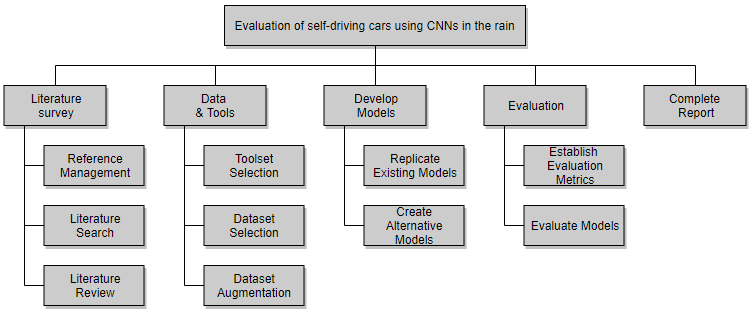
\includegraphics[width=1\linewidth]{figures/work-breakdown-structure.png}
\caption{Work Breakdown Structure}
\label{fig:workplan}
\end{figure}

%     \begin{tikzpicture}[
      every node/.style = {draw, rounded corners=3pt, semithick, drop shadow},
            ROOT/.style = {top color=green!60!blue, bottom color=blue!60!green,
                             inner sep=2mm, text=white, font=\bfseries},
              L1/.style = {fill=blue!20},
              L2/.style = {fill=orange!30},
              L3/.style = {fill=green!30, grow=down, xshift=1em, anchor=west, 
      edge from parent path={(\tikzparentnode.south) |- (\tikzchildnode.west)}},
edge from parent/.style = {draw, thick},
              LD/.style = {level distance=#1ex},
             LD1/.style = {level distance=6ex},
             LD2/.style = {level distance=12ex},
             LD3/.style = {level distance=18ex},
         level 1/.style = {sibling distance=32mm}
                        ]
    % Parents
\node[ROOT] {\begin{tabular}{c} This node \\ is \\ valuable \end{tabular}}
    [edge from parent fork down]
    child{node[L2] {AAA AAA AAA}
      child[L3,LD1]   {node[L3]   {A1}}
      child[L3,LD2]  {node[L3]   {A2}}
      child[L3,LD3]   {node[L3]   {A3}}
            }
    child{node[L2] {BB  BB BB BB}
      child[L3,LD1]  {node[L3]   {B1}}
      child[L3,LD2]  {node[L3]   {B2}}
            }
    child {node[L2] {C CC CCC}
      child[L3,LD1] {node[L3]   {C1}}
      child[L3,LD2] {node[L3]   {C2 C2 C2}
          child[L3,LD1] {node[L3,fill=red!30]   {C1}}
          child[L3,LD2] {node[L3,fill=red!30]   {C2}} 
                        }     
      child[L3,LD=30]  {node[L3]   {C2 C2 C2}}
            };
\end{tikzpicture}